%%%%%%%%%%%%%%%%%%%%%%%%%%%%%%%%%%%%%%%%%
% Short Sectioned Assignment LaTeX Template Version 1.0 (5/5/12)
% This template has been downloaded from: http://www.LaTeXTemplates.com
% Original author:  Frits Wenneker (http://www.howtotex.com)
% License: CC BY-NC-SA 3.0 (http://creativecommons.org/licenses/by-nc-sa/3.0/)
%%%%%%%%%%%%%%%%%%%%%%%%%%%%%%%%%%%%%%%%%

%----------------------------------------------------------------------------------------
%	PACKAGES AND OTHER DOCUMENT CONFIGURATIONS
%----------------------------------------------------------------------------------------

\documentclass[paper=a4, fontsize=11pt]{scrartcl} % A4 paper and 11pt font size

% ---- Entrada y salida de texto -----

\usepackage[T1]{fontenc} % Use 8-bit encoding that has 256 glyphs
\usepackage[utf8]{inputenc}
%\usepackage{fourier} % Use the Adobe Utopia font for the document - comment this line to return to the LaTeX default

% ---- Idioma --------

\usepackage[spanish, es-tabla]{babel} % Selecciona el español para palabras introducidas automáticamente, p.ej. "septiembre" en la fecha y especifica que se use la palabra Tabla en vez de Cuadro

\usepackage{fancyhdr}

% ---- Otros paquetes ----

\usepackage{amsmath,amsfonts,amsthm} % Math packages
%\usepackage{graphics,graphicx, floatrow} %para incluir imágenes y notas en las imágenes
\usepackage{graphics,graphicx, float} %para incluir imágenes y colocarlas

% Para hacer tablas comlejas
%\usepackage{multirow}
%\usepackage{threeparttable}

%\usepackage{sectsty} % Allows customizing section commands
%\allsectionsfont{\centering \normalfont\scshape} % Make all sections centered, the default font and small caps

\usepackage{fancyhdr} % Custom headers and footers
\usepackage{url}
\usepackage{hyperref}
%\usepackage{hyperref}
\pagestyle{fancyplain} % Makes all pages in the document conform to the custom headers and footers
\fancyhead{} % No page header - if you want one, create it in the same way as the footers below
\fancyfoot[L]{} % Empty left footer
\fancyfoot[C]{} % Empty center footer
\fancyfoot[R]{\thepage} % Page numbering for right footer
\renewcommand{\headrulewidth}{0pt} % Remove header underlines
\renewcommand{\footrulewidth}{0pt} % Remove footer underlines
\setlength{\headheight}{13.6pt} % Customize the height of the header

\numberwithin{equation}{section} % Number equations within sections (i.e. 1.1, 1.2, 2.1, 2.2 instead of 1, 2, 3, 4)
\numberwithin{figure}{section} % Number figures within sections (i.e. 1.1, 1.2, 2.1, 2.2 instead of 1, 2, 3, 4)
\numberwithin{table}{section} % Number tables within sections (i.e. 1.1, 1.2, 2.1, 2.2 instead of 1, 2, 3, 4)

\setlength\parindent{0pt} % Removes all indentation from paragraphs - comment this line for an assignment with lots of text

\newcommand{\horrule}[1]{\rule{\linewidth}{#1}} % Create horizontal rule command with 1 argument of height

\usepackage{booktabs}




%----------------------------------------------------------------------------------------
%	TÍTULO Y DATOS DEL ALUMNO
%----------------------------------------------------------------------------------------

\title{	
\normalfont \normalsize 
\textsc{{\bf Técnicas de los sistemas inteligentes (2014-2015)} \\ Grado en Ingeniería Informática \\ Universidad de Granada} \\ [25pt] % Your university, school and/or department name(s)
\horrule{0.5pt} \\[0.4cm] % Thin top horizontal rule
\huge  Práctica 3.1 - Planificación \\ % The assignment title
\horrule{2pt} \\[0.5cm] % Thick bottom horizontal rule
}

\author{Ignacio Martín Requena} % Nombre y apellidos

\date{\normalsize\today} % Incluye la fecha actual

%----------------------------------------------------------------------------------------
% DOCUMENTO
%----------------------------------------------------------------------------------------
\usepackage{graphicx}
\usepackage{listings}
\usepackage{color}
\definecolor{gray97}{gray}{.97}
\definecolor{gray75}{gray}{.75}
\definecolor{gray45}{gray}{.45}
 

\lstset{ frame=Ltb,
     framerule=0pt,
     aboveskip=0.5cm,
     framextopmargin=3pt,
     framexbottommargin=3pt,
     framexleftmargin=0.4cm,
     framesep=0pt,
     rulesep=.4pt,
     backgroundcolor=\color{gray97},
     rulesepcolor=\color{black},
     %
     stringstyle=\ttfamily,
     showstringspaces = false,
     basicstyle=\small\ttfamily,
     commentstyle=\color{gray45},
     keywordstyle=\bfseries,
     %
     numbers=left,
     numbersep=15pt,
     numberstyle=\tiny,
     numberfirstline = false,
     breaklines=true,
   }
 


\lstdefinestyle{consola}
   {basicstyle=\scriptsize\bf\ttfamily,
    backgroundcolor=\color{gray75},
   }
 
\lstdefinestyle{C}
   {language=C,
   }



\begin{document}

\maketitle % Muestra el Título

\newpage %inserta un salto de página

\tableofcontents % para generar el índice de contenidos

\listoffigures

%\listoftables

\newpage




%----------------------------------------------------------------------------------------
%	Cuestion 1
%----------------------------------------------------------------------------------------
\section{Ejercicio 1}

\subsection{Enunciado}

Escribir un dominio de planificación en PDDL para que un planificador pueda encontrar planes  de  actuación  para  uno  o  varios  robots  como  soluciones  a  problemas  de distribución de paquetes entre habitaciones. En el material de esta sesión de prácticas hay un fichero ejemplo de un problema para este tipo de dominio, que se corresponde con el estado inicial y objetivo en la figura de más abajo. Probar que el dominio escrito genera  plan  para  distintos  problemas (definidos  por  el  alumno) en  los  que  varíe  la cantidad  de  robots,la  cantidad  de  paquetes  a  distribuir  y  la  cantidad  de  habitaciones conectadas.

\subsection{Solución}

Para la resolución de este problema se ha implementado:
\begin{itemize}

	\item \textbf{Elementos}: tres elementos: un objeto, un paquete, un robot y una habitacion.

	\item \textbf{Predicados}: para representar si un objeto está en una habitación (at), si una habitación está conectada con otra (conectada), si el robot no posee nada (vacio) y si el robot esta llevando un paquete (llevando).
	
	\item \textbf{Acciones}: se han definido tres acciones:
	

	\begin{itemize}
	
		\item \textbf{Acción mover:} necesaria para representar el movimiento llevado a cabo por el robot para desplazar un paquete de una habitacion a otra.
		
		\item \textbf{Acción soltar:} que define el hecho de que el robot puede soltar ?obj en la habitación ?h
		
		\item \textbf{Acción coger:} para definir la acion de coger un paquete de una habitación por parte del robot
	
	\end{itemize}	

	
\end{itemize}


	En general el procedimiento seguido para el desarrollo de este problema ha sido el de pensar cuales eran las acciones necesarias para realizar el plan completo de mover un objeto de una habitación conectada a otra. \\
	\newpage
\subsection{Comprobación de la solución}

El problema utilizado para comprobar la solución de que el dominio implementado es correcto ha sido:

\begin{figure}[h]
\centering
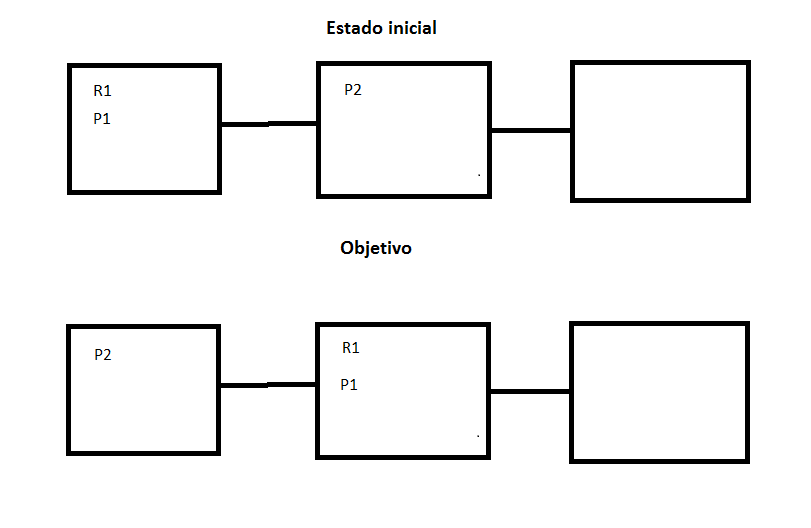
\includegraphics[width=1\linewidth]{p1}
\caption{Representación estado inicial y objetivo problema 1 dominio 1}
\label{fig:p1}
\end{figure}


	\begin{lstlisting}[language=SH]
(define (problem RDistribuye-1)
(:domain RobotDistribuidor)
(:objects
	r1 - robot
	p1 - paquete
	p2 - paquete
	
	hab0 - habitacion
	hab1 - habitacion
	hab2 - habitacion

	)
(:init
	(at r1 hab0)
	(at p1 hab0)
	(at p2 hab2)
	
	(vacio r1)
	
	(conectada hab0 hab1)
	(conectada hab1 hab0)
	(conectada hab2 hab1)
	(conectada hab1 hab2)
)
(:goal (and
	(at r1 hab1)
	(at p2 hab0)
	(at p1 hab2)
	))
)
	\end{lstlisting}
	
	He decidido escoger una solución con un robot, dos paquetes y tres habitaciones. Otra modificación respecto al fichero original proporcionado como ejemplo ha sido la de incluir en el estado inicial el hecho de que el robot no posee nada al principio (sin esta condición inicial el plan falla).


%----------------------------------------------------------------------------------------
%	Cuestion 2
%----------------------------------------------------------------------------------------

\section{Ejercicio 2}

\subsection{Enunciado}
Escribir un dominio de planificación
en  PDDL,  modificando el  dominio  del  anterior ejercicio, de tal manera  que  se  tenga  en  cuenta  que  la  acción  de  moverse  de  una habitación a otra consume una cantidad de batería y, por tanto, requiere que el robot tenga nivel de batería para moverse. Además, considerar que hay una nueva acción de carga  de  batería que  permite  reponer  la  batería.  Considerar  para  ello  que  se  ha definido un predicado (cambio n1 n2–nivelbat) que representa un cambio en el nivel de batería desde un nivel n1 a un nivel n2. En el material de esta sesión de prácticas hay un fichero ejemplo de un problema para este tipo de dominio.

\subsection{Solución}


Para la resolución de este problema se ha partido de la solución proporcionada en el ejercicio 1 realizando algunas modificaciones. En concreto, las modificaciones han sido:
\begin{itemize}

	\item \textbf{Elementos}: Se ha añadido un nuevo tipo de objeto para representar la existencia de la funte de bateria (fuente)

	\item \textbf{Predicados}: Se han añadido dos nuevos predicados para representar le cambio de la batería y el nivel de esta.
	
	\item \textbf{Acciones}: 

	\begin{itemize}
	
		\item \textbf{Acción mover:} En la acción mover se han añadido dos nuevos parámetros de tipo fuente, la batería antes y después. También se han modificado las precondiciones y los efectos de esta para representar el desgaste de la batería. 
		
	
	\end{itemize}	

	
\end{itemize}


	En general el procedimiento seguido para el desarrollo de este problema ha sido el de determinar cuando el nivel de batería debería bajar (en la acción de mover) asi como que estados de batería son necesarios representar (el de antes y el de despues de la carga). \\
	
	Lo que influye en la cantidad y niveles de batería definidos en el estado inicial es, basicamente, la colocación de las baterías y a que bateria tiene acceso cada robot.
	

\subsection{Comprobación de la solución}

El problema utilizado para comprobar la solución de que el dominio implementado es correcto ha sido:

\begin{figure}[h]
	\centering
	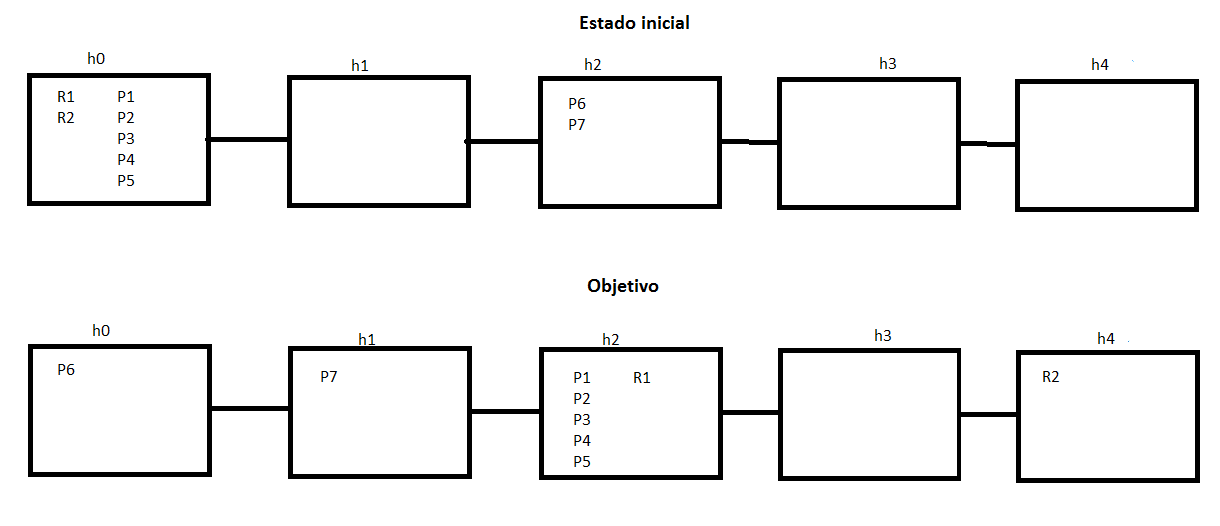
\includegraphics[width=1\linewidth]{p2}
	\caption{Representación estado inicial y objetivo problema 1 dominio 2}
	\label{fig:p1}
\end{figure}

	\begin{lstlisting}[language=SH]
(define (problem RDistribuye-1)
	(:domain RobotDistribuidor)
	(:objects
		r1 r2 - robot
		p1 p2 p3 p4 p5 p6 p7 - paquete
		hab0 hab1 hab2 hab3 hab4 - habitacion
		f0 f1 f2 - fuente
	)
	(:init
		(at r1 hab0)
		(at r2 hab0)
		(at p1 hab0)
		(at p2 hab0)
		(at p3 hab0)
		(at p4 hab0)
		(at p5 hab0)
		(at p6 hab2)
		(at p7 hab2)
		
		(vacio r1)
		(vacio r2)
		
		(nivelbateria r1 f2)
		(nivelbateria r2 f2)
		
		(cambio f2 f1)
		(cambio f1 f0)
		(cambio f0 f2)
		
		(conectada hab0 hab1)
		(conectada hab1 hab0)
		(conectada hab2 hab1)
		(conectada hab1 hab2)
		(conectada hab3 hab2)
		(conectada hab2 hab3)
		(conectada hab3 hab4)
		(conectada hab4 hab3)
	)
	(:goal (and
		(at p6 hab0)
		(at p7 hab1)
		(at p1 hab2)
		(at p2 hab2)
		(at p3 hab2)
		(at p4 hab2)
		(at p5 hab2)
		(at r1 hab2)
		(at r2 hab4)
		)
	)

)
	\end{lstlisting}
	
En este caso se ha optado por elegir un problema con dos robots, siete paquetes, cuatro habitaciones y 3 fuentes. Las habitaciones conetadas son: Habitacion 0 con 1, habitación 1 con 2, habitación 2 con 3 y habitación 3 con 4. A su vez las fuentes se pueden cambiar de la forma: f2 a f1, f1 a f0 y f0 a f2.
\newpage
%----------------------------------------------------------------------------------------
%	Cuestion 3
%----------------------------------------------------------------------------------------

\section{Ejercicio 3}

\subsection{Enunciado}

Escribir  un  dominio  de  planificación  en  PDDL,  modificando  el  dominio  del  anterior ejercicio,  de  manera  que  se  puedan  utilizar  ahora  dos acciones  diferentes,  moverse rápido y moverse lento tales que moverse rápido consume más unidades de fuel que moverse lento. Probarlo con varios problemas.

\subsection{Solución}


Para la resolución de este problema se ha tomado como base para la implementación la solución adoptada en el problema anterior. Los principales cambios con respecto a este han sido:
\begin{itemize}

	\item \textbf{Predicados}: Se ha añadido un nuevo predicado para representar el cambio en el nivel de la batería si el movimiento de nuestro robot es rápido.
	
	\item \textbf{Acciones}: Se ha añadido una nueva acción:

	\begin{itemize}
	
		\item \textbf{Acción mover rápido:} Esta acción tiene como objetivo simular el cambio en el nivel de batería de forma más rápida que si el robot se moviera a velocidad normal. Para ello se ha seguido el mismo esquema que para la accion mover a velocidad normal pero a la hora de representarel cambio en el nivel de la batería se ha usado el nuevo predicado cambio-rapido.
		
	
	\end{itemize}	

	
\end{itemize}


	En general el procedimiento seguido para el desarrollo de este problema ha sido el de pensar qué añadido tenía el hecho de que la velocidad del robot condicionara el nivel de batería llegando a la conclusión de que únicamente añadiendo un nuevo predicado para representar este hecho era suficiente. \\

\subsection{Comprobación de la solución}

Los problemas utilizados para comprobar la solución de que el dominio implementado es correcto han sido:

\begin{itemize}
	\item \textbf{Problema 1:}

\begin{figure}[h]
	\centering
	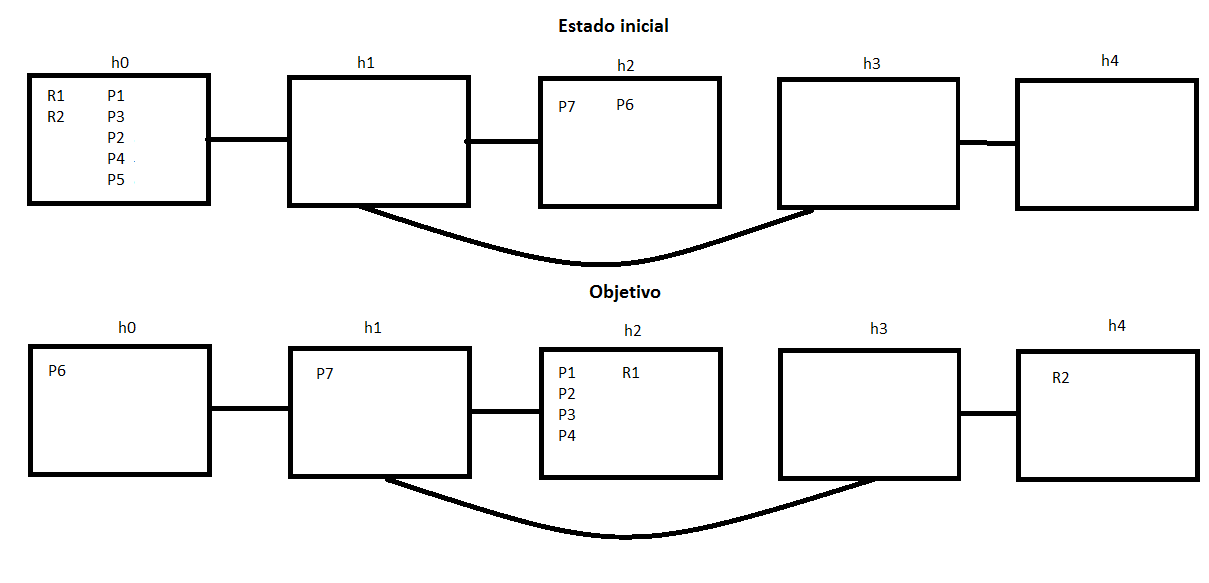
\includegraphics[width=1\linewidth]{p3-1}
	\caption{Representación estado inicial y objetivo problema 1 dominio 3}
	\label{fig:p1}
\end{figure}

	\begin{lstlisting}[language=SH]

(define (problem RDistribuye-1)
	(:domain RobotDistribuidor)
	(:objects
	r1 r2 - robot
	p1 p2 p3 p4 p5 p6 p7 p8 p9 p10 - paquete
	hab0 hab1 hab2 hab3 hab4 - habitacion
	fl1 fl2 fl0 - fuente
	)
	(:init
	(at r1 hab0)
	(at r2 hab0)
	
	(at p1 hab0)
	(at p3 hab0)
	(at p2 hab0)
	(at p4 hab0)
	(at p5 hab0)
	(at p7 hab2)
	(at p6 hab2)
	
	(vacio r1)
	(vacio r2)
	
	(nivelbateria r1 fl2)
	(nivelbateria r2 fl2)
	
	
	(cambio fl2 fl1)
	(cambio fl1 fl0)
	(cambio fl0 fl2)
	
	(cambio-rapido fl2 fl0)
	(cambio-rapido fl0 fl2)
	
	(conectada hab1 hab0)
	(conectada hab0 hab1)
	(conectada hab1 hab2)
	(conectada hab2 hab1)
	(conectada hab3 hab1)
	(conectada hab1 hab3)
	(conectada hab4 hab3)
	(conectada hab3 hab4)
	)
	
	(:goal (and
	(at p1 hab2)
	(at p3 hab2)
	(at p4 hab2)
	(at p2 hab2)
	(at p5 hab2)
	(at p6 hab0)
	(at p7 hab0)
	
	(at r1 hab2)
	(at r2 hab4)
	))

)

	\end{lstlisting}
	
En este caso se ha optado por elegir un problema con dos robots, siete paquetes, cuatro habitaciones y 3 fuentes. Las habitaciones conetadas son: Habitacion 0 con 1, habitación 1 con 2, habitación 2 con 3 y habitación 3 con 4. A su vez las fuentes se pueden cambiar de la forma: f2 a f1, f1 a f0 y f0 a f2.
\newpage
	\item \textbf{Problema 2}:
	
	\begin{figure}[h]
		\centering
		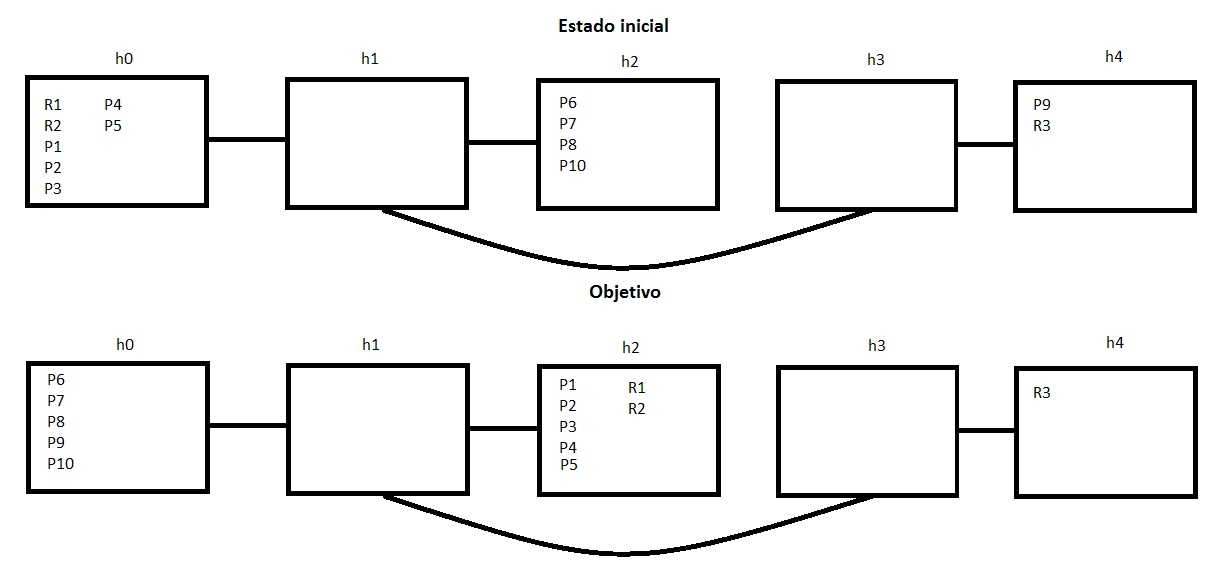
\includegraphics[width=1\linewidth]{p3-2}
		\caption{Representación estado inicial y objetivo problema 2 dominio 3}
		\label{fig:p1}
	\end{figure}
	
	\begin{lstlisting}[language=SH]
(define (problem RDistribuye-1)
(:domain RobotDistribuidor)
(:objects
	r1 r2 r3 - robot
	p1 p2 p3 p4 p5 p6 p7 p8 p9 p10 - paquete
	hab0 hab1 hab2 hab3 hab4 - habitacion
	fl1 fl2 fl3 - fuente
	)
(:init
	(at r1 hab0)
	(at r2 hab0)
	(at r3 hab4)
	
	(at p1 hab0)
	(at p2 hab0)
	(at p3 hab0)
	(at p4 hab0)
	(at p5 hab0)
	(at p6 hab2)
	(at p7 hab2)
	(at p8 hab2)
	(at p9 hab4)
	(at p10 hab2)

	(vacio r1)
	(vacio r2)
	(vacio r3)

	(nivelbateria r1 fl2)
	(nivelbateria r2 fl2)
	(nivelbateria r3 fl2)

	(cambio fl3 fl2)
	(cambio fl2 fl1)
	(cambio fl1 fl2)

	(cambio-rapido fl2 fl3)
	(cambio-rapido fl1 fl2)

	(conectada hab0 hab1)
	(conectada hab1 hab0)
	(conectada hab2 hab1)
	(conectada hab1 hab2)
	(conectada hab1 hab3)
	(conectada hab3 hab1)
	(conectada hab3 hab4)
	(conectada hab4 hab3)
)
(:goal (and
	(at p1 hab2)
	(at p2 hab2)
	(at p3 hab2)
	(at p4 hab2)
	(at p6 hab0)
	(at p5 hab2)
	(at p7 hab0)
	(at p8 hab0)
	(at p9 hab0)
	(at p10 hab0)

	(at r1 hab2)
	(at r2 hab2)
	(at r3 hab4)
	))

)

\end{lstlisting}

En este segundo problema implementado se ha intentado complicar el estado inicial. Este estado está compuesto por tres robots, dos de ellos en la habitación 0 y uno en la 4; cuatro habitaciones, diez paquetes y tres fuentes de batería.

\end{itemize}

\newpage
%----------------------------------------------------------------------------------------
%	Cuestion 4
%----------------------------------------------------------------------------------------

\section{Ejercicio 4}

\subsection{Enunciado}

Escribir  un  dominio  de  planificación  en  PDDL  2.1  que  responda  a  los  requisitos explicados  en  los  anteriores  ejercicios, utilizando  las  capacidades  expresivas  de  PDDL 2.1,  es  decir,  representando  funciones  numéricas.  Al  igual  que  en  los  anteriores ejercicios,   definir   distintos   problemas   para   comprobar   que   vuestro   dominio  es correcto.

\subsection{Solución}


Para la resolución de este problema se ha modificado el dominio del problema 3 para representar la carga y descarga del robot a través de funciones numéricas en lugar de a través de predicados. En concreto los elementos añadidos y modificados con respecto al problema anterior han sido:
\begin{itemize} 

	\item \textbf{Predicados}: Se han eliminado los predicados que representaban el cambio de batería del robot así como la carga y descarga. Esto es porque la representación de este estado se ha realizado mediante funciones.
	
	\item \textbf{Funciones}: Se ha añadido una función (descarga) que representa el agotamiento de la batería
	
	\item \textbf{Acciones}: Se han modificado y/o añadido las acciones:

	\begin{itemize}
	
		\item \textbf{Acción mover y mover rápido:} Se han modificado estas dos acciones con una llamada a la función descarga que, en función de si la acción es mover o mover rápido el nivel de la batería se decrementa en 5 o en 10 respectivamente.
		
		\item \textbf{Acción cargar}: Esta nueva acción representa el momento en el que el robot se carga. Como precondición he definido que el nivel de batería sea menor a 5 y, una vez cargado el robot, este nivel aumenta hasta 50 (es decir, se carga completamente)
	
	\end{itemize}	

	
\end{itemize}


	En general el procedimiento seguido para el desarrollo de este problema ha sido el de sustituir los anteriores objetos y predicados del problema que representaban el estado de la batería por una función numérica que representa la misma situación. A partir de esto se han modificado y añadido las acciones pertinentes para el control de la misma. \\
\newpage
\subsection{Comprobación de la solución}

Los problemas utilizados para comprobar la solución de que el dominio implementado es correcto han sido:

\begin{itemize}

\item \textbf{Problema 1:}

\begin{figure}[h]
	\centering
	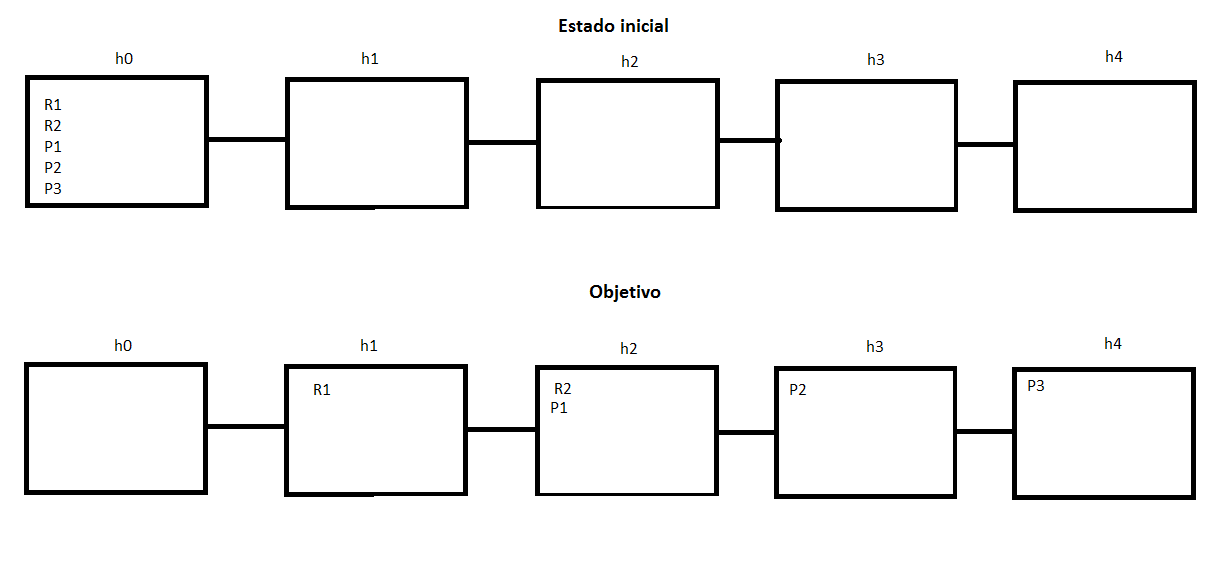
\includegraphics[width=1\linewidth]{p4-1}
	\caption{Representación estado inicial y objetivo problema 1 dominio 4}
	\label{fig:p1}
\end{figure}

	\begin{lstlisting}[language=SH]
(define (problem RDistribuye-1)
(:domain RobotDistribuidor)
(:objects
	r1 r2 - robot
	p1 p2 p3 p4 p5 p6 p7 - paquete
	hab0 hab1 hab2 hab3 hab4 - habitacion
	)
(:init
	(at r1 hab0)
	(at r2 hab0)
	(at p1 hab0)
	(at p2 hab0)
	(at p3 hab0)

	(vacio r1)
	(vacio r2)
	
	(= (descarga r1 ) 50)
	(= (descarga r2 ) 50)
	
	(conectada hab0 hab1)
	(conectada hab1 hab0)
	(conectada hab2 hab1)
	(conectada hab1 hab2)
	(conectada hab2 hab3)
	(conectada hab3 hab2)
	(conectada hab3 hab4)
	(conectada hab4 hab3)
)
(:goal (and
	(at p1 hab2)
	(at p2 hab3)
	(at p3 hab4)
	
	(at r1 hab1)
	(at r2 hab2)
	))

)
	\end{lstlisting}

En este dominio se han usado 2 robots, 7 paquetes y 5 habitaciones. 


\item\textbf{ Problema 2:}

En este segundo problema implementado se ha añadido un nuevo robot posicionado junto a un único paquete con el fin de comprobar si PDDL resuelve de forma eficiente el problema, es decir, utiliza el robot 3 para mover el paquete 9 y no hace ir a otro robot a por el. A demás se han definido 10 paquetes y 5 habitaciones.\\

\begin{figure}[h]
	\centering
	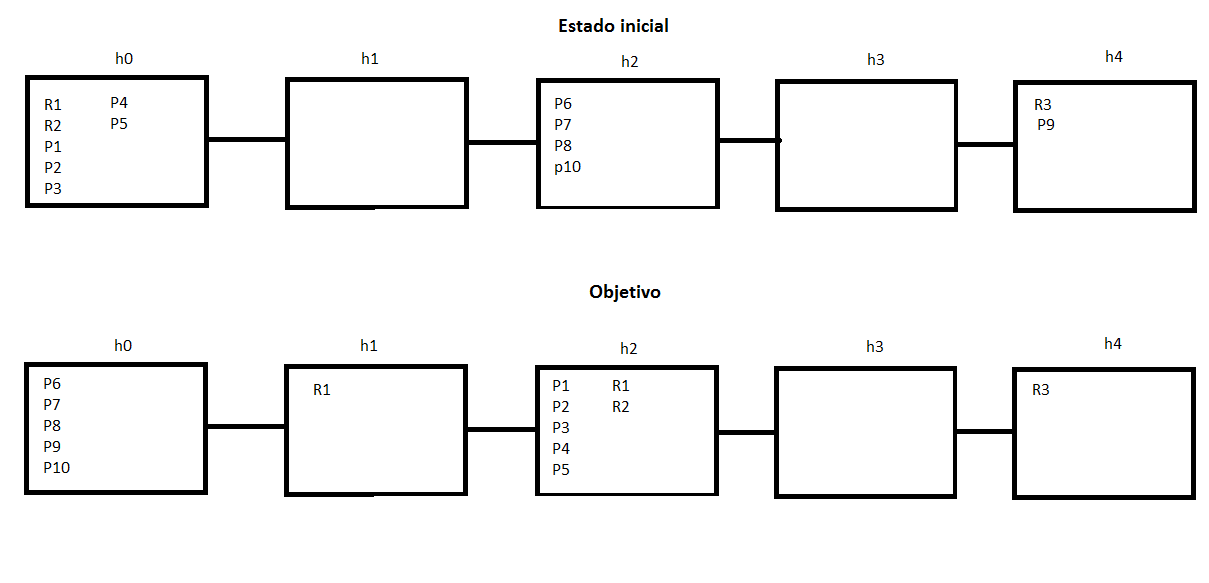
\includegraphics[width=1\linewidth]{p4-2}
	\caption{Representación estado inicial y objetivo problema 2 dominio 4}
	\label{fig:p4-2}
\end{figure}

	\begin{lstlisting}[language=SH]
(define (problem RDistribuye-1)
(:domain RobotDistribuidor)
(:objects
	r1 r2 r3 - robot
	p1 p2 p3 p4 p5 p6 p7 p8 p9 p10 - paquete
	hab0 hab1 hab2 hab3 hab4 - habitacion
	)
(:init
	(at r1 hab0)
	(at r2 hab0)
	(at r3 hab4)
	(at p1 hab0)
	(at p2 hab0)
	(at p3 hab0)
	(at p4 hab0)
	(at p5 hab0)
	(at p6 hab2)
	(at p7 hab2)
	(at p8 hab2)
	(at p9 hab4)
	(at p10 hab2)

	(vacio r1)
	(vacio r2)
	(vacio r3)

	(= (descarga r1 ) 50)
	(= (descarga r2 ) 50)
	(= (descarga r3 ) 50)

	(conectada hab0 hab1)
	(conectada hab1 hab0)
	(conectada hab2 hab1)
	(conectada hab1 hab2)
	(conectada hab1 hab3)
	(conectada hab3 hab1)
	(conectada hab3 hab4)
	(conectada hab4 hab3)
)
(:goal (and
	(at p6 hab0)
	(at p7 hab0)
	(at p8 hab0)
	(at p9 hab0)
	(at p10 hab0)
	(at p1 hab2)
	(at p2 hab2)
	(at p3 hab2)
	(at p4 hab2)
	(at p5 hab2)

	(at r1 hab2)
	(at r2 hab2)
	(at r3 hab4)
	))

)

	\end{lstlisting}
	
	
	
\item \textbf{Problema 3:}

Este tercer y último problema ha sido una variación del representado en la\textbf{ Figura \ref{fig:p4-2}}. En concreto se ha añadido un robot mas y se ha cambiado el estado objetivo para complicar aún más el problema (aun así el planificador Metric-FF solo ha necesitado 54 pasos para resolverlo).

\begin{figure}[h]
	\centering
	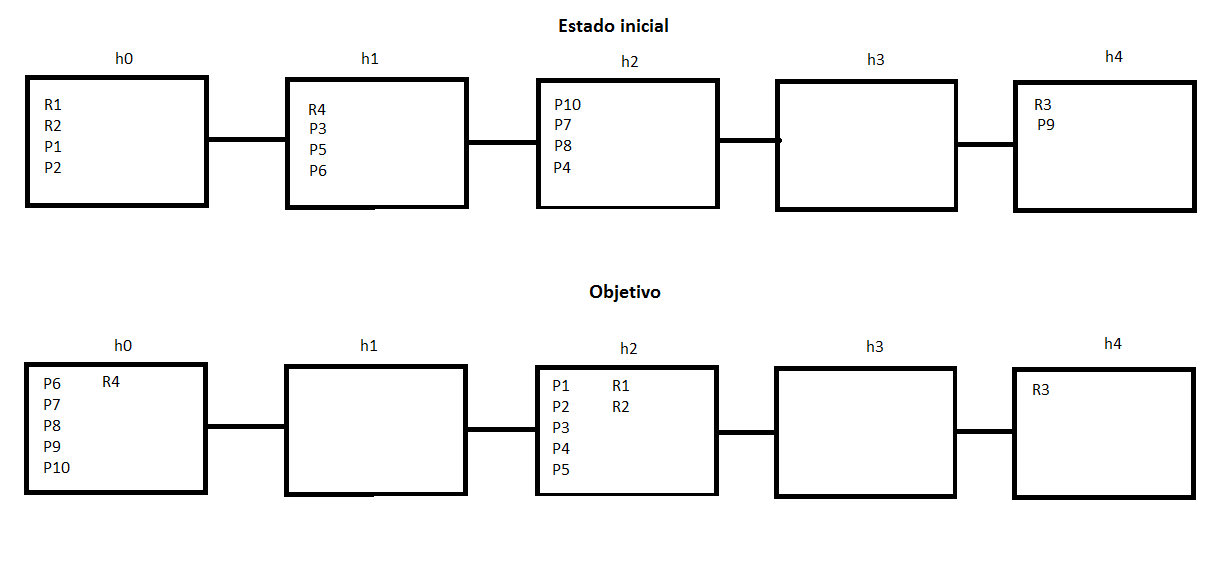
\includegraphics[width=1\linewidth]{p4-3}
	\caption{Representación estado inicial y objetivo problema 3 dominio 4}
	\label{fig:p1}
\end{figure}

	\begin{lstlisting}[language=SH]

(define (problem RDistribuye-1)
(:domain RobotDistribuidor)
(:objects
	r1 r2 r3 r4 - robot
	p1 p2 p3 p4 p5 p6 p7 p8 p9 p10 - paquete
	hab0 hab1 hab2 hab3 hab4 - habitacion
	)
(:init
	(at r1 hab0)
	(at r2 hab0)
	(at r3 hab4)
	(at r4 hab1)

	(at p1 hab0)
	(at p2 hab0)
	(at p3 hab1)
	(at p4 hab2)
	(at p5 hab1)
	(at p6 hab1)
	(at p7 hab2)
	(at p8 hab2)
	(at p9 hab4)
	(at p10 hab2)

	(vacio r1)
	(vacio r2)
	(vacio r3)
	(vacio r4)


	(= (descarga r1 ) 50)
	(= (descarga r2 ) 50)
	(= (descarga r3 ) 50)
	(= (descarga r4 ) 50)


	(conectada hab0 hab1)
	(conectada hab1 hab0)
	(conectada hab2 hab1)
	(conectada hab1 hab2)
	(conectada hab1 hab3)
	(conectada hab3 hab1)
	(conectada hab3 hab4)
	(conectada hab4 hab3)
)
(:goal (and
	(at p6 hab0)
	(at p7 hab0)
	(at p8 hab0)
	(at p9 hab0)
	(at p10 hab0)
	(at p1 hab2)
	(at p2 hab2)
	(at p3 hab2)
	(at p4 hab2)
	(at p5 hab2)

	(at r1 hab2)
	(at r2 hab2)
	(at r3 hab4)
	(at r4 hab0)
	))

)

	\end{lstlisting}

\end{itemize}

\end{document}